\section{Sensorik}
Eine zentrale Aufgabe besteht darin die Zustandsgrößen zu messen, um den geschlossenen Regelkreis berechnen zu können. Deshalb beschäftigt sich der folgende Abschnitt mit der verwendeten Sensorik und derer Auswertung. Hierfür müssen die Sensoren zuerst in das Modell eingebunden werden um Messkennlinien zu bestimmen. Daraufhin werden die Empfindlichkeiten untersucht und Rückschlüsse auf den Aufbau gezogen. Zusätzlich muss die Diskretisierung durch die Sensoren untersucht werden um ungewollte Abtasteffekte zu vermeiden. Zuletzt werden die Störeinflüsse analysiert und Ansätze präsentiert um diese zu verringern.

\begin{figure}[!h]
\centering
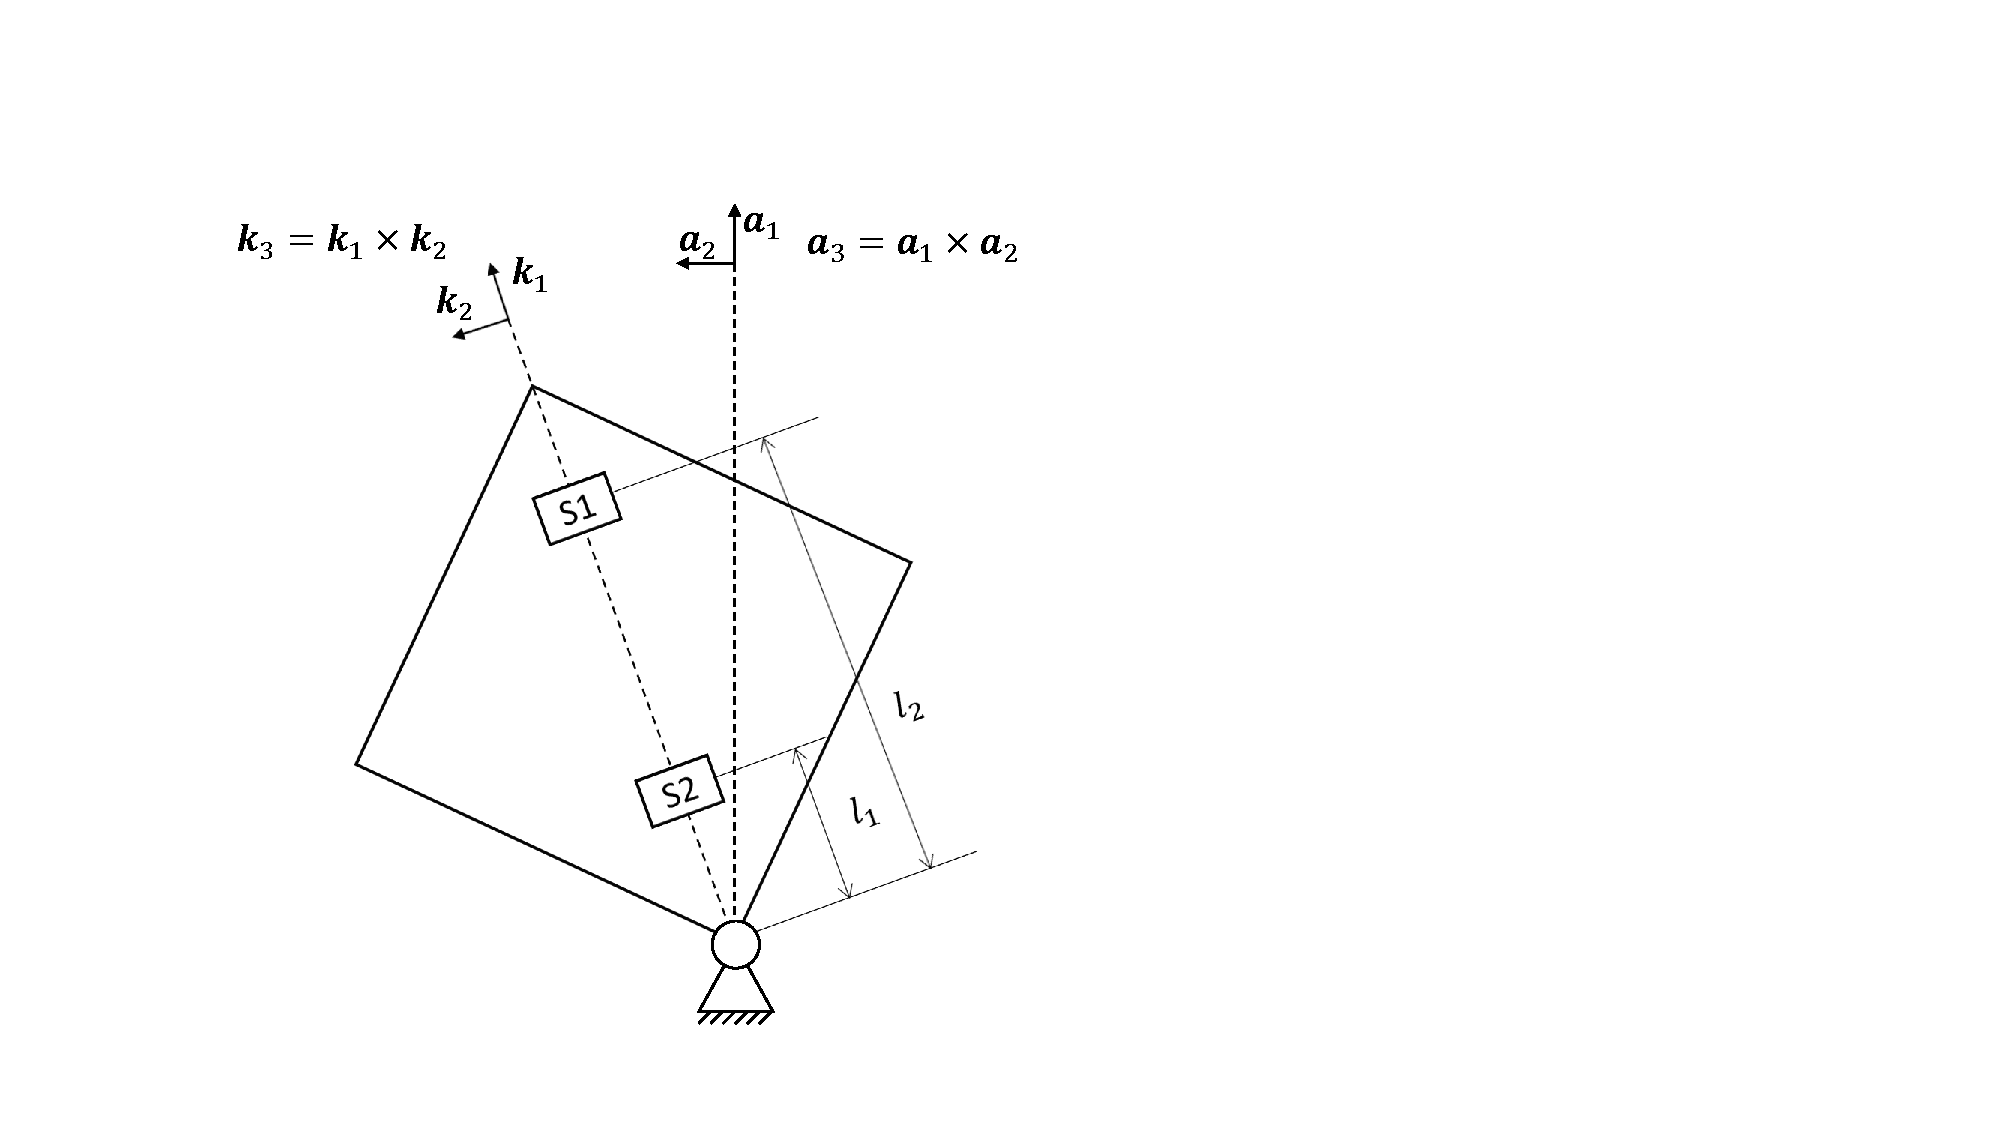
\includegraphics[width=0.6\linewidth, trim={1cm 1.5cm 18cm 3.5cm}, clip]{3_Sensorik/img/SensorAnordnung}
\caption{Anordnung der Sensoren an der Würfelseite, Quelle: eigene Darstellung}
\end{figure}

An der Würfelseite sind zwei MPU6050-ICs angebracht, um die Größen $\varphi$, $\dot{\varphi}$ und $\ddot{\varphi}$ zu messen. Die ICs verfügen über einen Beschleunigungs- und Drehratensensor, welche jeweils Messwerte in Richtung von drei Achsen liefern. Zuerst müssen Messkennlinien ermittelt werden. Das heißt die Messwerte der Sensoren werden mit Hilfe des mechanischen Modells in Zusammenhang mit den Messgrößen $\varphi$, $\dot{\varphi}$ und $\ddot{\varphi}$ gebracht. 

Die Messwerte der Drehratensensoren entsprechen der Winkelgeschwindigkeit der Würfelseite im körperfesten Bezugssystem $K$.

\begin{equation}
\bs{\omega}_{S_i} = \begin{pmatrix}
\omega^{S_i}_x \\ \omega^{S_i}_y \\ \omega^{S_i}_z
\end{pmatrix} = \presuper{K}{\big(\vel{A}{\omega}{K}\big)} = \begin{pmatrix}
{0} \\ {0} \\ {\dot{\varphi}}
\end{pmatrix}
\end{equation}

Somit sind nur die Komponenten in Richtung der Z-Achse von Bedeutung. Diese werden als Messwerte $y_i$ definiert.

\begin{equation}
y_i \equiv \omega^{S_i}_z \hspace{35pt} y_i = \dot{\varphi} \hspace{35pt} (i=1, 2)
\end{equation}

Die Ausgabewerte $\bs{a}_{S_i}$ der Beschleunigungssensoren setzt sich, nach dem idealisierten Modell, aus zwei Termen zusammen. Der erste Term entspricht der Beschleunigung der Sensoren im raumfesten Bezugssystem $A$, welche gleich der zweiten Ableitung des Ortvektors $\bs{s}_i$ der Sensoren mit Respekt zu $A$ ist.

\begin{equation}
\begin{split}
\vel{A}{a}{S_i} &= \frac{\presuper{A}{d} \vel{A}{v}{S_i}}{dt} = \frac{\presuper{A}{d}}{dt}\big(\vel{A}{\bs{\omega}}{K} \times \bs{s}_i\big) = \frac{\presuper{A}{d}\vel{A}{\omega}{K}}{dt}\times \bs{s}_i + \vel{K}{\omega}{S_i} \times \frac{\presuper{A}{d}\bs{s}_i}{dt} \\
&= \vel{K}{\alpha}{S_i} \times \bs{s}_i + \vel{A}{\omega}{K} \times \big(\vel{A}{\omega}{K} \times \bs{s}_i\big)
\\
&= \vecBS{K}{0}{0}{\ddot{\varphi}} \times \vecBS{K}{l_i}{0}{0}  + \vecBS{K}{0}{0}{\dot{\varphi}} \times \begin{pmatrix}
\vecBS{K}{0}{0}{\dot{\varphi}} \times \vecBS{K}{l_i}{0}{0} 
\end{pmatrix} = \vecBS{K}{-\dot{\varphi}^2 \cdot l_i}{\ddot{\varphi}\cdot l_i}{0}
\end{split}
\end{equation}

Der zweite Term wird von der Gravitation beeinflusst. Das heißt er entspricht der Darstellung des Erdbeschleunigungsvektors im körperfesten Bezugssystem $K$.

\begin{equation}
\bs{g} = \pMat{A}{K} \cdot \vecBS{A}{-g}{0}{0} = \vecBS{K}{-g \cdot c_{\varphi}}{g \cdot s_{\varphi}}{0}
\end{equation}

Somit ergeben sich die folgenden Zusammenhänge für die Anzeigewerte $\bs{a}_{S_i}$ der Beschleunigungssensoren, welche wiederum als Messwerte $y_3,...,y_6$ definiert werden.

\begin{equation}
\bs{a}_{S_i} = \begin{pmatrix}
\ddot{x}_{S_i} \\ \ddot{y}_{S_i} \\ \ddot{z}_{S_i}
\end{pmatrix} = 
\presuper{K}{\big(\vel{A}{a}{S_i} + \bs{g}\big)} = \vecBS{K}{-\dot{\varphi}^2 \cdot l_i - g\cdot c_{\varphi}}{\ddot{\varphi}\cdot l_i + g \cdot s_{\varphi}}{0}
\end{equation}
\begin{equation}
\begin{split}
&y_3 \equiv a^{S_1}_x \hspace{35pt} y_3 = -\dot{\varphi}^2 \cdot l_1 - g \cdot c_{\varphi} \\
&y_4 \equiv a^{S_2}_x \hspace{35pt} y_4 = -\dot{\varphi}^2  \cdot l_2 - g\cdot c_{\varphi} \\
&y_5 \equiv a^{S_1}_y \hspace{35pt} y_5 = \ddot{\varphi} \cdot l_1 + g\cdot s_{\varphi} \\
&y_6 \equiv a^{S_2}_y \hspace{35pt} y_6 = \ddot{\varphi} \cdot l_2 + g\cdot s_{\varphi}
\end{split}
\end{equation}

Die Messwerte der Beschleunigungssensoren hängen jeweils von zwei Messgrößen ab. Deshalb ist es nicht möglich aus einem einzelnen Messwert einen Rückschluss auf die Messgrößen zu ziehen. Allerdings ist der Einfluss des Winkels $\varphi$ unabhängig von dem Abstand $l_i$ des Sensors zum Drehpunkt. Folglich kann dieser Anteil durch die Differenz von zwei Messwerten eliminiert werden.
\begin{equation}
\begin{split}
&y_7 \equiv y_3 - y_4 \hspace{35pt} y_7 = -\dot{\varphi}^2 \cdot (l_1 - l_2) \\
&y_8 \equiv y_5 - y_6 \hspace{35pt} y_8 = \ddot{\varphi} \cdot (l_1 - l_2)
\end{split}
\end{equation}
Analog können die Messwerte $y_9$ und $y_10$ definiert werden um die Messgröße $\varphi$ zu ermitteln. In diesem Fall wird der Subtrahend mit dem Verhältnis der Sensorabstände zum Drehpunkt gewichtet.
\begin{equation}
\begin{split}
y_9 \equiv y_3 - \frac{l_1}{l_2}y_4 &\hspace{35pt} y_9 = -g \cdot c_{\varphi} \cdot (1 - \frac{l_1}{l_2}) \\
y_{10} \equiv y_5 - \frac{l_1}{l_2}y_6 &\hspace{35pt} y_{10} = g \cdot s_{\varphi} \cdot (1 - \frac{l_1}{l_2}) \\
y_{11} \equiv \frac{y_{10}}{y_9}  &\hspace{35pt} y_{11} = -tan(\varphi)
\end{split}
\end{equation}
Die verschiedenen Kennlinien zeigen, dass mehrere Möglichkeiten bestehen um die Messgrößen $\varphi$, $\dot{\varphi}$ und $\ddot{\varphi}$ mit den Messwerten in Verbindung zu bringen. Folglich müssen nun Kriterien erarbeitet werden um die Messsysteme beurteilen zu können. Zuerst ist hier die Empfindlichkeit $S$ zu nennen, welche wiedergibt wie stark sich eine Änderung der Messgröße auf den zugehörigen Messwert auswirkt. Die Berechnung der Empfindlichkeit erfolgt über die partielle Ableitung der Kennlinie nach der Messgröße. Somit ergeben sich für die Messwerte, welche von dem Winkel $\varphi$ abhängen, die folgenden Empfindlichkeiten.
\begin{equation}
\begin{split}
S_9(\varphi) &= \frac{\partial y_9}{\partial \varphi} = g\cdot s_{\varphi}\cdot (1 - \frac{l_1}{l_2}) \\
S_{10}(\varphi) &= \frac{\partial y_{10}}{\partial \varphi} = g \cdot c_{\varphi} \cdot (1- \frac{l_1}{l_2}) \\
S_{11}(\varphi) &= \frac{\partial y_{11}}{\partial \varphi} = -tan(\varphi)^2 - 1
\end{split}
\end{equation}
\begin{figure}[h!]
\centering
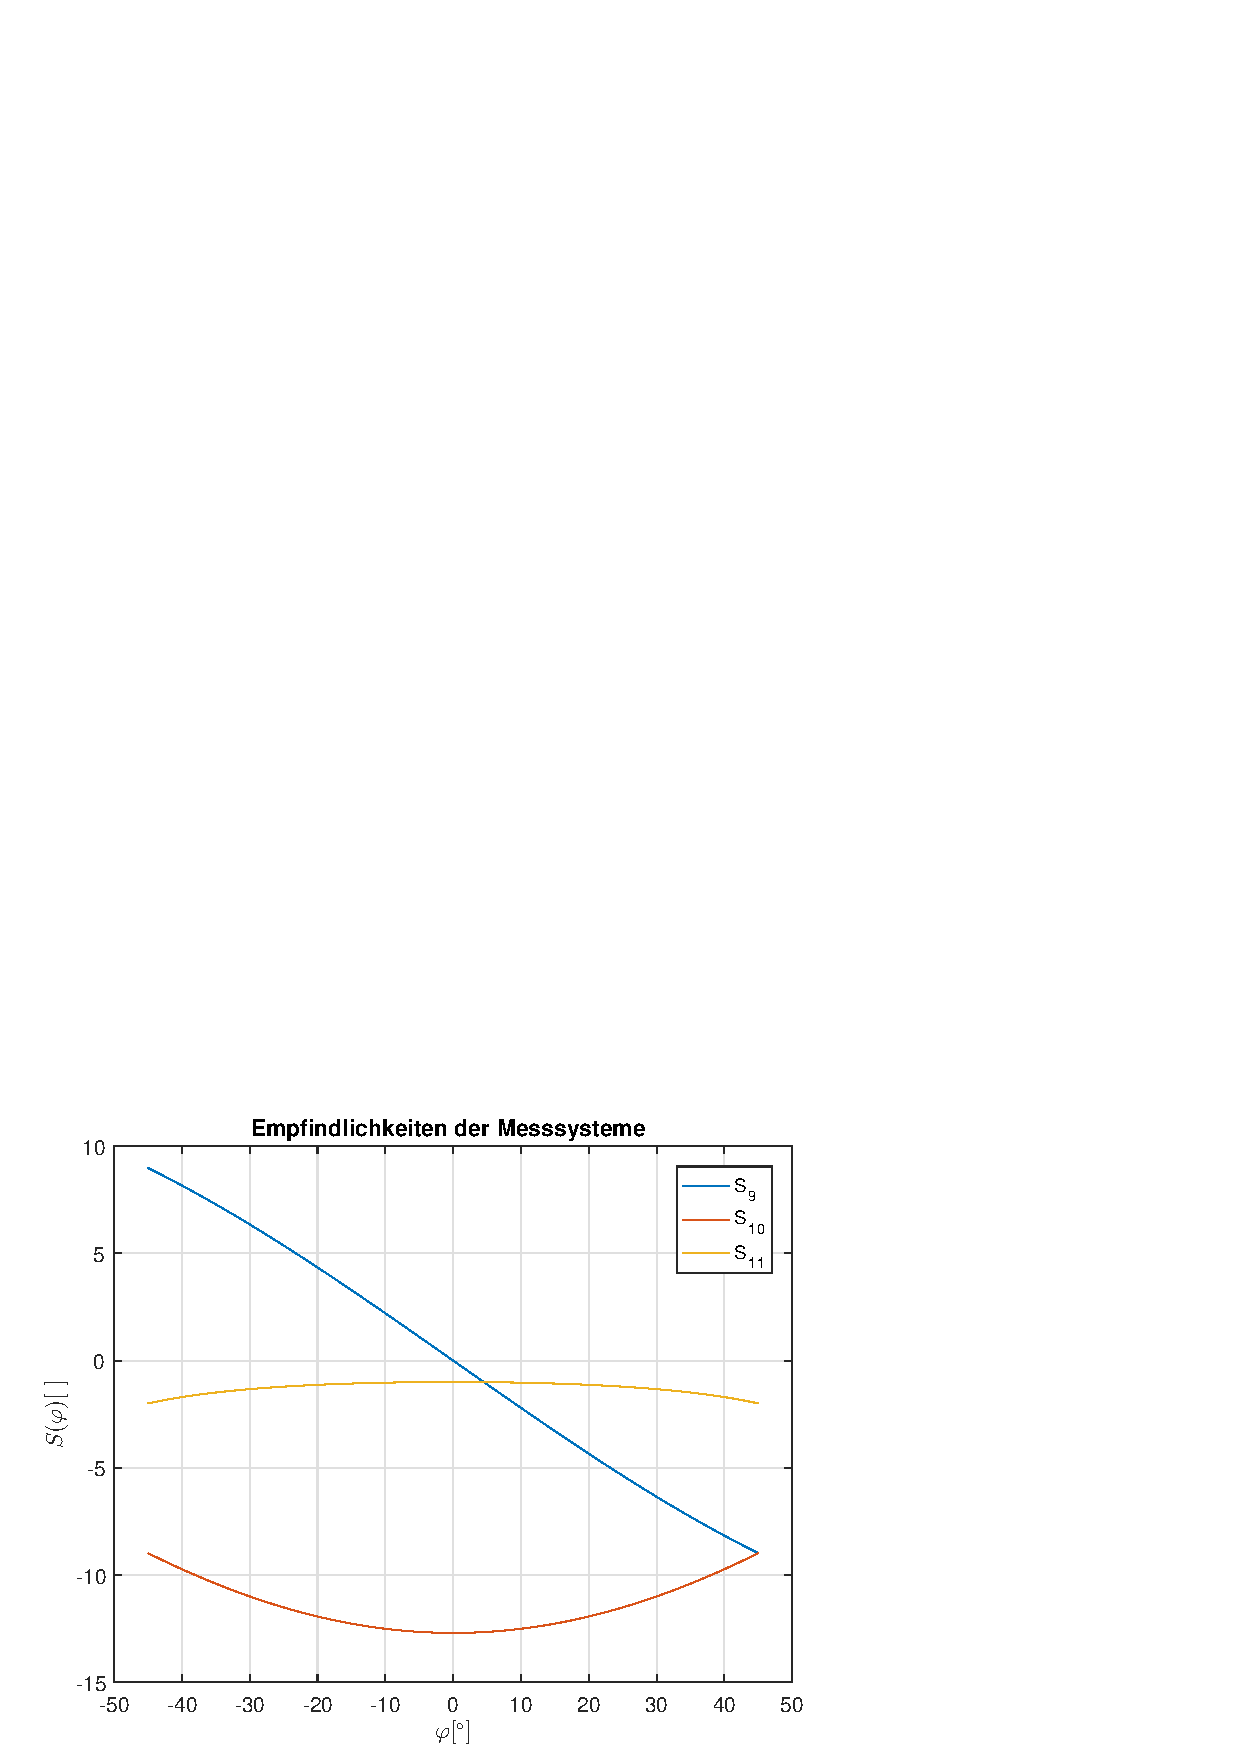
\includegraphics[width=0.5\linewidth]{3_Sensorik/img/empfindlichkeit_phi}
\caption{Empfindlichkeiten für $\varphi$, Quelle: eigene Darstellung}
\end{figure}
Aus der obigen Abbildungen ist leicht zu erkennen, dass der Messwert $y_{10}$ die höchste Empfindlichkeit besitzt. Besonders im Arbeitsbereich der Regelung ($\varphi=0$) liegt das Maximum der Empfindlichkeit. Das heißt bereits kleine Änderung des Winkels $\varphi$ führen zu einer merkbaren Anpassung des Messwertes $y_{10}$. Die Empfindlichkeit $S_{11}$ ist zwar deutlich geringer, weist allerdings nahezu konstante Werte im Arbeitsbereich der Regelung auf, was wiederum für eine lineare Messkennlinie in diesem Bereich spricht. Aus den Gleichung lässt sich zusätzlich erkenne, dass die Empfindlichkeiten $S_9$ und $S_{10}$ von der Positionen der Sensoren abhängt. Hieraus folgt, das die Empfindlichkeit der Messwerte $y_9$ und $y_{10}$, mit zunehmendem $l_1$ und abnehmendem $l_2$, steigt.

Die Messgröße $\dot{\varphi}$ beeinflusst lediglich zwei Messwerte, nämlich $y_1$ und $y_7$. Hierbei sei angemerkt, dass $y_7$ proportional zu dem Quadrat von $\dot{\varphi}$ ist und somit lediglich der Betrag der Messgröße aus dem Wert rekonstruiert werden kann. Die Information über die Richtung muss aus einer anderen Quelle gewonnen werden. 
\begin{equation}
\begin{split}
S_1 &= S_2 = \frac{\partial y_1}{\partial \dot{\varphi}} = 1 \\
S_7 &= \frac{\partial y_7}{\partial \dot{\varphi}} = -2\cdot \dot{\varphi}\cdot (l_1 - l_2)
\end{split}
\end{equation}
\begin{figure}[h!]
\centering
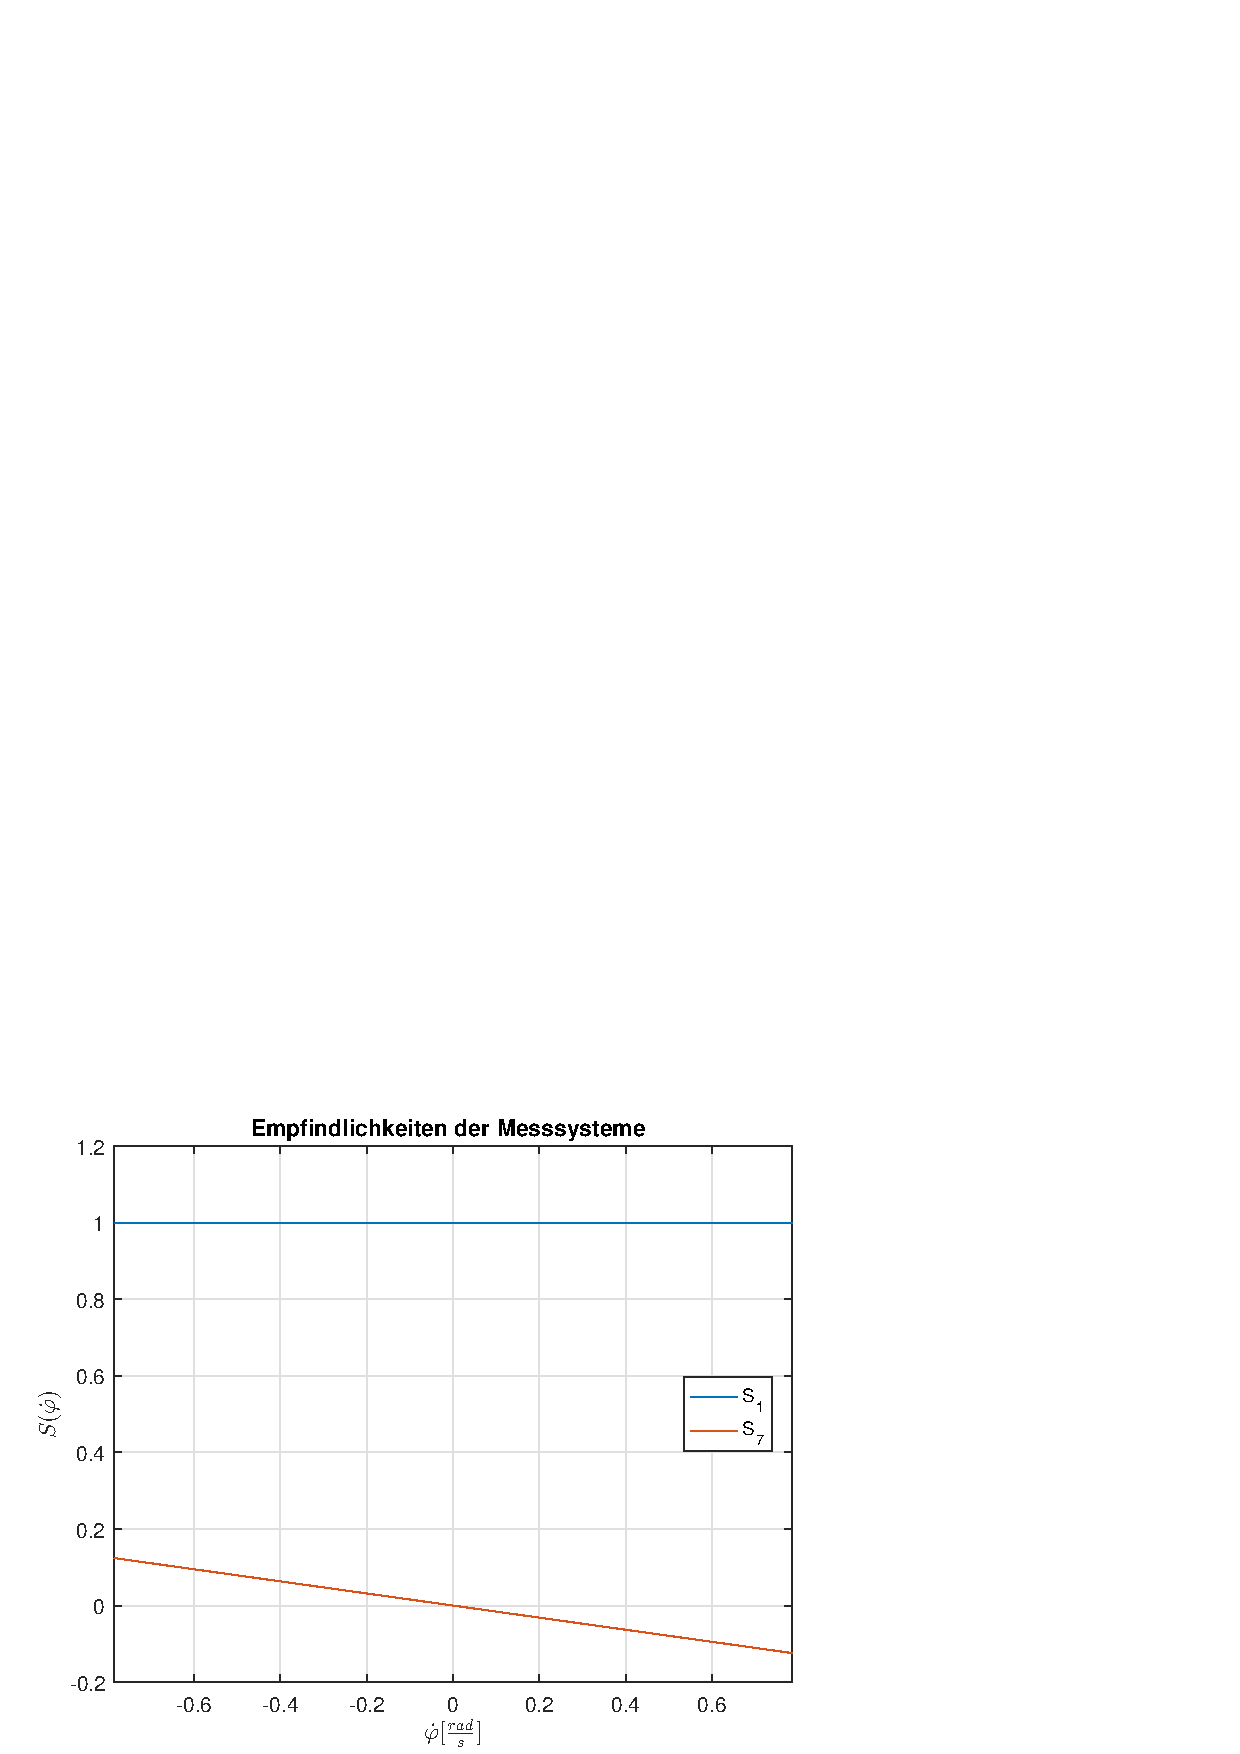
\includegraphics[width=0.5\linewidth]{3_Sensorik/img/empfindlichkeit_phi__d}
\caption{Empfindlichkeiten für $\dot{\varphi}$, Quelle: eigene Darstellung}
\end{figure}
Der Graph zeigt deutlich, dass die Empfindlichkeiten $S_1$ und $S_2$ der Drehratensensoren höher sind als die der Geschwindigkeitsschätzung mit Hilfe der Beschleunigungssensoren. Lediglich bei hohen Werten von $\dot{\varphi}$ erreicht man mit Hilfe von $y_7$ eine höhere Empfindlichkeit.

\newpage
Zuletzt ist der Messwert $y_8$ zu untersuchen, welcher als einziger von der Messgröße $\ddot{\varphi}$ abhängt. Hierbei handelt es sich um eine konstante Kennlinie bzw. einer konstanten Empfindlichkeit, welche wiederum mit zunehmenden Abstand zwischen den beiden Sensoren steigt.

\begin{equation}
S_8 = \frac{\partial y_8}{\partial \ddot{\varphi}} = l_1 - l_2
\end{equation}

\begin{figure}[h!]
\centering
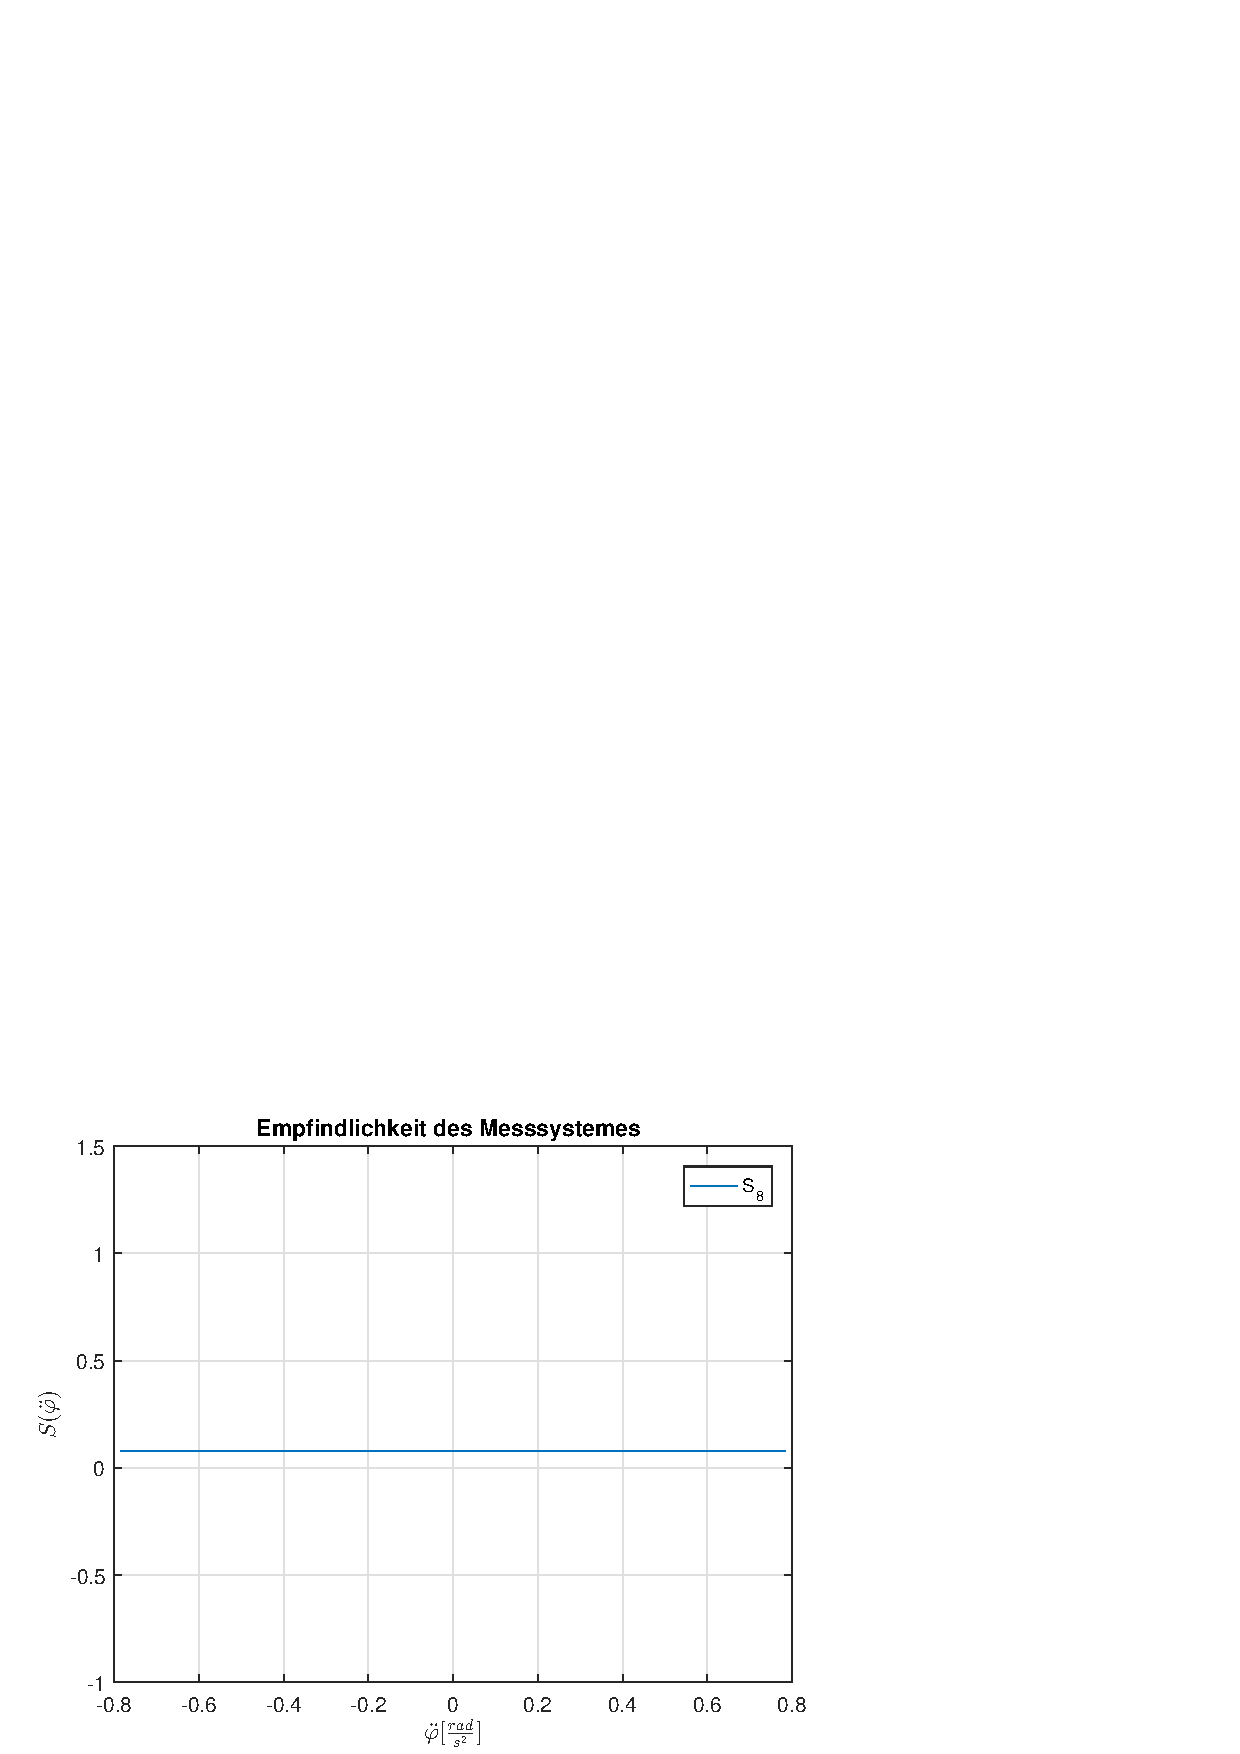
\includegraphics[width=0.5\linewidth]{3_Sensorik/img/empfindlichkeit_phi__dd}
\caption{Empfindlichkeit für $\ddot{\varphi}$, Quelle: eigene Darstellung}
\end{figure}

Das erste Fazit aus der Untersuchung ist, dass alle Empfindlichkeiten, die von der Position der Sensoren abhängen, mit zunehmendem Abstand der Sensoren zueinander, wachsen. Folglich muss $l_1$ möglichst groß und $l_2$ möglichst klein gewählt werden.